\documentclass{article}
\usepackage[spanish]{babel}
\usepackage{graphicx}
\usepackage{geometry}

\geometry{
    top=2cm,
    bottom=2cm,
    left=2cm,
    right=2cm
}

\title{Actividad 2}
\author{}

\begin{document}

\maketitle

\hspace{1cm} El sistema analizado anteriormente presenta alguanas carencias, dicho modelo solo considera el caso en el que solamente una especie vive en el entorno. Pero la realidad es más compleja 
que eso, es así que nos disponemos a introducir a el modelo una nueva especie. Ahora consideramos las poblaciones de especies distintas \(N_1\) y \(N_2\), además, los nuevos parámetros 
\(\alpha_{ij}\) se refieren a el coeficiente de competencia interespecífica de la especie \(j\) sobre la especie \(i\):

\begin{equation}
\frac {dN_1} {dt} = r_1N_1 \frac {K_1 - N_1 - \alpha_{12}N_2} {K_1} \label{eq:(1)}
\end{equation}
\begin{equation}
\frac {dN_2} {dt} = r_2N_2 \frac {K_2 - N_2 - \alpha_{21}N_1} {K_2} \label{eq:(2)}
\end{equation}

\hspace{1cm} Esta nueva dinámica de poblaciones, conocida como el modelo de competencia de Lotka-Volterra, constituye un nuevo sistema de ecuaciones diferenciales ordinarias. En las expresiones, 
\(r_i\) sigue siendo la tasa de crecimiento intrínseca de la especie \(i\) y \(K_i\), la capacidad de carga de la especie \(i\). 

\hspace{1cm} En este caso, el sistema de ecuaciones diferenciales ordinarias es más complejo, pero aún podemos asegurar la existencia y unicidad de la solución. Para ello, observamos que ambas
ecuaciones \ref{eq:(1)} y \ref{eq:(2)} son continuas por lo que nos disponemos a verificar que cumplan la Condición de Lipschitz.IMPORTANTE: ACA HAY QUE VER QUE EL SISTEMA DE ODES TIENE SOLUCIÓN ÚNICA. 

\hspace{1cm} Nos encontramos que para esta dinámica, las soluciones de \(N_1(t)\) y \(N_2(t)\) no son triviales como sí sucedía en el experimento anterior. Es así que decidimos aprovechar las comparaciones
que realizamos anteriormente entre los distintos métodos numéricos para aproximar de manera más precisa las soluciones de este nuevo sistema de ecuaciones diferenciales ordinarias. Los resultados 
del experimento anterior nos sugieren que la mejor aproximación la obtendremos con el método de Runge-Kutta de orden 4 utilizando un paso de integración de \(h = 0.01\). 

\hspace{1cm} Antes de representar las series temporales de las poblaciones de las especies, nos centramos en analizar la dinámica general del sistema. Para ello, consideramos las curvas en las que
\(dN_1/dt = 0\) y \(dN_2/dt = 0\). Estas curvas, conocidas como las isoclinas o nuclinas nos permiten entender las cantidades de cada población en la que la tasa de crecimiento de alguna especie
es nula. Además, nos permiten identificar los puntos de equilibrio del sistema, es decir, aquellos puntos en los que la tasa de crecimiento de ambas especies es nula. De la ecuación \ref{eq:(1)}
obtenemos que la isoclina para \(N_1\) es:
\begin{equation}
N_1 = K_1 - \alpha_{12}N_2 \label{eq:(3)}
\end{equation}
\hspace{1cm} De la misma manera, de la ecuación \ref{eq:(2)} obtenemos que la isoclina para \(N_2\) es:
\begin{equation}
N_2 = K_2 - \alpha_{21}N_1  \label{eq:(4)}
\end{equation}
\hspace{1cm} De las ecuaciones \ref{eq:(3)} y \ref{eq:(4)} podemos observar que las isoclinas son rectas en el plano \(N_1N_2\). Asimismo, si nos atenemos al modelo de competencia de Lotka-Volterra,
entonces tanto \(\alpha_{12}\) como \(\alpha_{21}\) son positivos, por lo que las isoclinas tendrán pendiente negativa. Esto implica que las soluciones pueden ser de cuatro formas distintas
dependiendo de los parámetros \(K_1\), \(K_2\), \(\alpha_{12}\) y \(\alpha_{21}\). Gráficos genéricos para estos casos se presentan a continuación:
\begin{figure*}
    \centering
    \makebox[\textwidth][c]{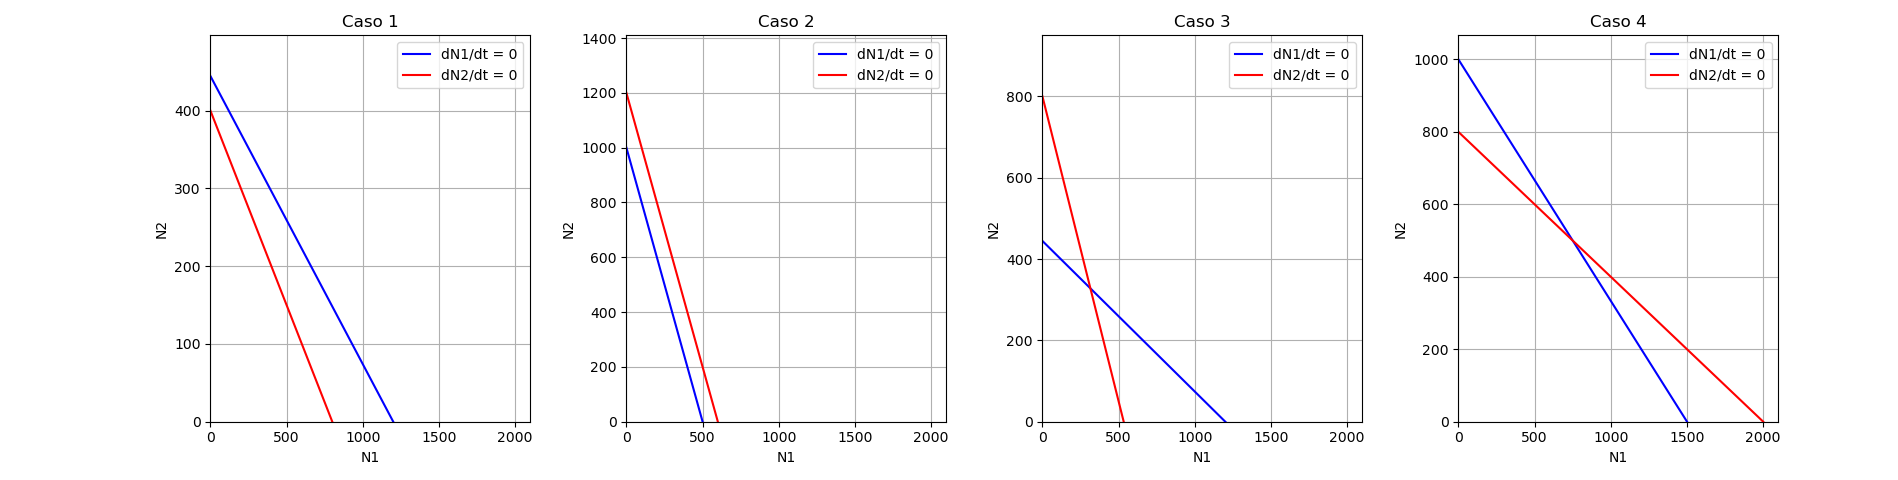
\includegraphics[width=1.4\textwidth]{tipos_de_isoclinas.png}}
    \caption{Distintos tipos de dinámicas dependiendo de los valores relativos de \(K_1\), \(K_2\), \(\alpha_12\) y \(\alpha_21\)}
    \label{fig:imagen-larga}
\end{figure*}
\hspace{1cm}Como se puede observar en la figura \ref{fig:imagen-larga}, existen cuatro posibles dinámicas para el sistema de ecuaciones diferenciales ordinarias.
 En el caso en el que \(\frac {K_1}{\alpha_12} > K_2\) y \(K_1 > \frac {K_2}{\alpha_{21}}\) situación a la que llamaremos caso 1 así como cuando 
\(\frac {K_1}{\alpha_12} < K_2\) y \(K_1 < \frac {K_2}{\alpha_{21}}\), nuestro caso 2, observamos que no hay ningún punto de equilibrio en el sistema. Es posible
llegar a dicha conclusión dado que las isoclinas no se intersecan, en otras palabras, no hay un punto en el que ambas tasas de crecimiento sean nulas. Por otro lado, 
en el caso en el que \(\frac {K_1}{\alpha_12} > K_2\) y \(K_1 < \frac {K_2}{\alpha_{21}}\), caso 3, y cuando \(\frac {K_1}{\alpha_12} < K_2\) y 
\(K_1 > \frac {K_2}{\alpha_{21}}\), caso 4, observamos que hay un punto de equilibrio en el sistema. En estos casos, el punto de equilibrio se ubica en la intersección
de las isoclinas:

\end{document}